\section{Sonogram Class Reference}
\label{classSonogram}\index{Sonogram@{Sonogram}}
{\tt \#include $<$sonogram.h$>$}

Inheritance diagram for Sonogram:\begin{figure}[H]
\begin{center}
\leavevmode
\includegraphics[width=89pt]{classSonogram__inherit__graph}
\end{center}
\end{figure}
Collaboration diagram for Sonogram:\begin{figure}[H]
\begin{center}
\leavevmode
\includegraphics[width=89pt]{classSonogram__coll__graph}
\end{center}
\end{figure}


\subsection{Detailed Description}
\begin{Desc}
\item[Author:]Melchior FRANZ \end{Desc}




Definition at line 25 of file sonogram.h.\subsection*{Public Member Functions}
\begin{CompactItemize}
\item 
{\bf Sonogram} ({\bf QWidget} $\ast$)
\item 
{\bf $\sim$Sonogram} ()
\item 
void {\bf init} ()
\item 
void {\bf analyze} (const Scope \&)
\item 
void {\bf transform} (Scope \&)
\item 
void {\bf demo} ()
\item 
const QPixmap $\ast$ {\bf background} () const 
\item 
const QPixmap $\ast$ {\bf canvas} () const 
\item 
uint {\bf timeout} () const
\item 
uint {\bf height} () const
\end{CompactItemize}
\subsection*{Protected Member Functions}
\begin{CompactItemize}
\item 
QPixmap $\ast$ {\bf canvas} ()
\item 
void {\bf erase\-Canvas} ()
\item 
void {\bf paint\-Event} (QPaint\-Event $\ast$)
\item 
void {\bf resize\-Event} (QResize\-Event $\ast$)
\item 
void {\bf palette\-Change} (const class QPalette \&)
\item 
void {\bf polish} ()
\item 
void {\bf draw\-Frame} ()
\item 
virtual void {\bf paused} ()
\item 
void {\bf change\-Timeout} (uint new\-Timeout)
\end{CompactItemize}
\subsection*{Protected Attributes}
\begin{CompactItemize}
\item 
QTimer {\bf m\_\-timer}
\item 
uint {\bf m\_\-timeout}
\item 
uint {\bf m\_\-height}
\item 
{\bf FHT} {\bf m\_\-fht}
\end{CompactItemize}


\subsection{Constructor \& Destructor Documentation}
\index{Sonogram@{Sonogram}!Sonogram@{Sonogram}}
\index{Sonogram@{Sonogram}!Sonogram@{Sonogram}}
\subsubsection{\setlength{\rightskip}{0pt plus 5cm}Sonogram::Sonogram ({\bf QWidget} $\ast$)}\label{classSonogram_Sonograma0}




Definition at line 18 of file sonogram.cpp.



\footnotesize\begin{verbatim}18                                   :
19         Analyzer::Base2D(parent, 16)
20 {
21 setBackgroundColor(QColor(255,255,255));
22 }

\end{verbatim}\normalsize 
\index{Sonogram@{Sonogram}!~Sonogram@{$\sim$Sonogram}}
\index{~Sonogram@{$\sim$Sonogram}!Sonogram@{Sonogram}}
\subsubsection{\setlength{\rightskip}{0pt plus 5cm}Sonogram::$\sim${\bf Sonogram} ()}\label{classSonogram_Sonograma1}




Definition at line 25 of file sonogram.cpp.



\footnotesize\begin{verbatim}26 {
27 }
\end{verbatim}\normalsize 


\subsection{Member Function Documentation}
\index{Sonogram@{Sonogram}!analyze@{analyze}}
\index{analyze@{analyze}!Sonogram@{Sonogram}}
\subsubsection{\setlength{\rightskip}{0pt plus 5cm}void Sonogram::analyze (const Scope \&)\hspace{0.3cm}{\tt  [virtual]}}\label{classSonogram_Sonograma3}




Implements {\bf Analyzer::Base$<$ QWidget $>$} {\rm (p.\,\pageref{classAnalyzer_1_1Base_Analyzer_1_1Baseb3})}.

Definition at line 36 of file sonogram.cpp.

References Analyzer::Base2D::canvas(), and Analyzer::Base$<$ QWidget $>$::height().

Referenced by demo().



\footnotesize\begin{verbatim}37 {
38         int x = width() - 1;
39         QColor c;
40         
41         QPainter p(canvas());
42 
43         bitBlt(canvas(), 0, 0, canvas(), 1, 0, x, height());
44         //canvas()->fill();
45         Scope::const_iterator it = s.begin();
46         for (int y = height() - 1; y && it < s.end(); it++) {
47                 if (*it < .005)
48                         c = backgroundColor();
49                 else if (*it < .05)
50                         c.setHsv(95, 255, 255 - int(*it * 4000.0));
51                 else if (*it < 1.0)
52                         c.setHsv(95 - int(*it * 90.0), 255, 255);
53                 else
54                         c = Qt::red;
55 
56                 p.setPen(c);
57                 p.drawPoint(x, y--);
58         }
59 }
\end{verbatim}\normalsize 


Here is the call graph for this function:\begin{figure}[H]
\begin{center}
\leavevmode
\includegraphics[width=176pt]{classSonogram_Sonograma3_cgraph}
\end{center}
\end{figure}
\index{Sonogram@{Sonogram}!background@{background}}
\index{background@{background}!Sonogram@{Sonogram}}
\subsubsection{\setlength{\rightskip}{0pt plus 5cm}const QPixmap$\ast$ Analyzer::Base2D::background () const\hspace{0.3cm}{\tt  [inline, inherited]}}\label{classAnalyzer_1_1Base2D_Sonograma6}




Definition at line 75 of file analyzerbase.h.

References Analyzer::Base2D::m\_\-background.

Referenced by Analyzer::Base2D::erase\-Canvas().



\footnotesize\begin{verbatim}75 { return &m_background; }
\end{verbatim}\normalsize 
\index{Sonogram@{Sonogram}!canvas@{canvas}}
\index{canvas@{canvas}!Sonogram@{Sonogram}}
\subsubsection{\setlength{\rightskip}{0pt plus 5cm}QPixmap$\ast$ Analyzer::Base2D::canvas ()\hspace{0.3cm}{\tt  [inline, protected, inherited]}}\label{classAnalyzer_1_1Base2D_Sonogramb0}




Definition at line 86 of file analyzerbase.h.

References Analyzer::Base2D::m\_\-canvas.



\footnotesize\begin{verbatim}86 { return &m_canvas; }
\end{verbatim}\normalsize 
\index{Sonogram@{Sonogram}!canvas@{canvas}}
\index{canvas@{canvas}!Sonogram@{Sonogram}}
\subsubsection{\setlength{\rightskip}{0pt plus 5cm}const QPixmap$\ast$ Analyzer::Base2D::canvas () const\hspace{0.3cm}{\tt  [inline, inherited]}}\label{classAnalyzer_1_1Base2D_Sonograma7}




Definition at line 76 of file analyzerbase.h.

References Analyzer::Base2D::m\_\-canvas.

Referenced by analyze(), Analyzer::Base2D::draw(), Analyzer::Base2D::erase\-Canvas(), and Analyzer::Base2D::paint\-Event().



\footnotesize\begin{verbatim}76 { return &m_canvas; }
\end{verbatim}\normalsize 
\index{Sonogram@{Sonogram}!changeTimeout@{changeTimeout}}
\index{changeTimeout@{changeTimeout}!Sonogram@{Sonogram}}
\subsubsection{\setlength{\rightskip}{0pt plus 5cm}void {\bf Analyzer::Base}$<$ {\bf QWidget}  $>$::change\-Timeout (uint {\em new\-Timeout})\hspace{0.3cm}{\tt  [inline, protected, inherited]}}\label{classAnalyzer_1_1Base_Analyzer_1_1Baseb6}




Definition at line 54 of file analyzerbase.h.



\footnotesize\begin{verbatim}55     {
56         m_timer.changeInterval( newTimeout );
57         m_timeout = newTimeout;
58     }
\end{verbatim}\normalsize 
\index{Sonogram@{Sonogram}!demo@{demo}}
\index{demo@{demo}!Sonogram@{Sonogram}}
\subsubsection{\setlength{\rightskip}{0pt plus 5cm}void Sonogram::demo ()\hspace{0.3cm}{\tt  [virtual]}}\label{classSonogram_Sonograma5}




Reimplemented from {\bf Analyzer::Base$<$ QWidget $>$} {\rm (p.\,\pageref{classAnalyzer_1_1Base_Analyzer_1_1Baseb5})}.

Definition at line 73 of file sonogram.cpp.

References analyze(), and FHT::size().



\footnotesize\begin{verbatim}74 {
75         analyze(Scope(m_fht.size(), 0));
76 }
\end{verbatim}\normalsize 


Here is the call graph for this function:\begin{figure}[H]
\begin{center}
\leavevmode
\includegraphics[width=241pt]{classSonogram_Sonograma5_cgraph}
\end{center}
\end{figure}
\index{Sonogram@{Sonogram}!drawFrame@{drawFrame}}
\index{drawFrame@{drawFrame}!Sonogram@{Sonogram}}
\subsubsection{\setlength{\rightskip}{0pt plus 5cm}void {\bf Analyzer::Base}$<$ {\bf QWidget}  $>$::draw\-Frame ()\hspace{0.3cm}{\tt  [protected, inherited]}}\label{classAnalyzer_1_1Base_Analyzer_1_1Baseb1}




Referenced by Analyzer::Base2D::draw().\index{Sonogram@{Sonogram}!eraseCanvas@{eraseCanvas}}
\index{eraseCanvas@{eraseCanvas}!Sonogram@{Sonogram}}
\subsubsection{\setlength{\rightskip}{0pt plus 5cm}void Analyzer::Base2D::erase\-Canvas ()\hspace{0.3cm}{\tt  [inline, protected, inherited]}}\label{classAnalyzer_1_1Base2D_Sonogramb1}




Definition at line 87 of file analyzerbase.h.

References Analyzer::Base2D::background(), and Analyzer::Base2D::canvas().

Referenced by init(), and Analyzer::Base2D::resize\-Event().



\footnotesize\begin{verbatim}87 { bitBlt( canvas(), 0, 0, background() ); }
\end{verbatim}\normalsize 


Here is the call graph for this function:\begin{figure}[H]
\begin{center}
\leavevmode
\includegraphics[width=195pt]{classAnalyzer_1_1Base2D_Sonogramb1_cgraph}
\end{center}
\end{figure}
\index{Sonogram@{Sonogram}!height@{height}}
\index{height@{height}!Sonogram@{Sonogram}}
\subsubsection{\setlength{\rightskip}{0pt plus 5cm}uint {\bf Analyzer::Base}$<$ {\bf QWidget}  $>$::height () const\hspace{0.3cm}{\tt  [inline, inherited]}}\label{classAnalyzer_1_1Base_Analyzer_1_1Basea1}




Definition at line 43 of file analyzerbase.h.

Referenced by analyze().



\footnotesize\begin{verbatim}43 { return m_height; }
\end{verbatim}\normalsize 
\index{Sonogram@{Sonogram}!init@{init}}
\index{init@{init}!Sonogram@{Sonogram}}
\subsubsection{\setlength{\rightskip}{0pt plus 5cm}void Sonogram::init ()\hspace{0.3cm}{\tt  [virtual]}}\label{classSonogram_Sonograma2}




Reimplemented from {\bf Analyzer::Base2D} {\rm (p.\,\pageref{classAnalyzer_1_1Base2D_Analyzer_1_1Base2Db1})}.

Definition at line 30 of file sonogram.cpp.

References Analyzer::Base2D::erase\-Canvas().



\footnotesize\begin{verbatim}31 {
32         eraseCanvas();
33 }
\end{verbatim}\normalsize 


Here is the call graph for this function:\begin{figure}[H]
\begin{center}
\leavevmode
\includegraphics[width=254pt]{classSonogram_Sonograma2_cgraph}
\end{center}
\end{figure}
\index{Sonogram@{Sonogram}!paintEvent@{paintEvent}}
\index{paintEvent@{paintEvent}!Sonogram@{Sonogram}}
\subsubsection{\setlength{\rightskip}{0pt plus 5cm}void Analyzer::Base2D::paint\-Event (QPaint\-Event $\ast$)\hspace{0.3cm}{\tt  [inline, protected, inherited]}}\label{classAnalyzer_1_1Base2D_Sonogramb2}




Definition at line 89 of file analyzerbase.h.

References Analyzer::Base2D::canvas(), and Analyzer::Base2D::m\_\-canvas.



\footnotesize\begin{verbatim}89 { if( !m_canvas.isNull() ) bitBlt( this, 0, 0, canvas() ); }
\end{verbatim}\normalsize 


Here is the call graph for this function:\begin{figure}[H]
\begin{center}
\leavevmode
\includegraphics[width=179pt]{classAnalyzer_1_1Base2D_Sonogramb2_cgraph}
\end{center}
\end{figure}
\index{Sonogram@{Sonogram}!paletteChange@{paletteChange}}
\index{paletteChange@{paletteChange}!Sonogram@{Sonogram}}
\subsubsection{\setlength{\rightskip}{0pt plus 5cm}void Analyzer::Base2D::palette\-Change (const class QPalette \&)\hspace{0.3cm}{\tt  [protected, inherited]}}\label{classAnalyzer_1_1Base2D_Sonogramb4}


\index{Sonogram@{Sonogram}!paused@{paused}}
\index{paused@{paused}!Sonogram@{Sonogram}}
\subsubsection{\setlength{\rightskip}{0pt plus 5cm}virtual void {\bf Analyzer::Base}$<$ {\bf QWidget}  $>$::paused ()\hspace{0.3cm}{\tt  [protected, virtual, inherited]}}\label{classAnalyzer_1_1Base_Analyzer_1_1Baseb4}


\index{Sonogram@{Sonogram}!polish@{polish}}
\index{polish@{polish}!Sonogram@{Sonogram}}
\subsubsection{\setlength{\rightskip}{0pt plus 5cm}void Analyzer::Base2D::polish ()\hspace{0.3cm}{\tt  [protected, inherited]}}\label{classAnalyzer_1_1Base2D_Sonogramb5}




Definition at line 159 of file analyzerbase.cpp.

References Analyzer::Base2D::init().



\footnotesize\begin{verbatim}160 {
161     //TODO is there much point in this anymore?
162 
163     //we use polish for initialzing (instead of ctor)
164     //because we need to know the widget's final size
165     QWidget::polish();
166 
167     init(); //virtual
168 }
\end{verbatim}\normalsize 


Here is the call graph for this function:\begin{figure}[H]
\begin{center}
\leavevmode
\includegraphics[width=159pt]{classAnalyzer_1_1Base2D_Sonogramb5_cgraph}
\end{center}
\end{figure}
\index{Sonogram@{Sonogram}!resizeEvent@{resizeEvent}}
\index{resizeEvent@{resizeEvent}!Sonogram@{Sonogram}}
\subsubsection{\setlength{\rightskip}{0pt plus 5cm}void Analyzer::Base2D::resize\-Event (QResize\-Event $\ast$)\hspace{0.3cm}{\tt  [protected, inherited]}}\label{classAnalyzer_1_1Base2D_Sonogramb3}




Definition at line 171 of file analyzerbase.cpp.

References Analyzer::Base2D::erase\-Canvas(), Analyzer::Base2D::m\_\-background, and Analyzer::Base2D::m\_\-canvas.



\footnotesize\begin{verbatim}172 {
173     m_height = QWidget::height();
174     m_background.resize( size() );
175     m_canvas.resize( size() );
176 
177     #ifdef DRAW_GRID
178     QPainter p( &m_background );
179     p.setPen( QColor( 0x20, 0x20, 0x50 ) );
180 
181     for( uint x = 0, w = m_background.width(), h = m_background.height()-1;
182         x < w; x += 3 ) p.drawLine( x, 0, x, h );
183     for( uint y = 0, w = m_background.width()-1 , h = m_background.height();
184         y < h; y += 3 ) p.drawLine( 0, y, w, y );
185     #else
186     m_background.fill( backgroundColor() );
187     #endif
188 
189     eraseCanvas(); //this is necessary
190 
191     QWidget::resizeEvent( e );
192 }
\end{verbatim}\normalsize 


Here is the call graph for this function:\begin{figure}[H]
\begin{center}
\leavevmode
\includegraphics[width=291pt]{classAnalyzer_1_1Base2D_Sonogramb3_cgraph}
\end{center}
\end{figure}
\index{Sonogram@{Sonogram}!timeout@{timeout}}
\index{timeout@{timeout}!Sonogram@{Sonogram}}
\subsubsection{\setlength{\rightskip}{0pt plus 5cm}uint {\bf Analyzer::Base}$<$ {\bf QWidget}  $>$::timeout () const\hspace{0.3cm}{\tt  [inline, inherited]}}\label{classAnalyzer_1_1Base_Analyzer_1_1Basea0}




Definition at line 42 of file analyzerbase.h.

Referenced by Analyzer::Base2D::Base2D().



\footnotesize\begin{verbatim}42 { return m_timeout; }
\end{verbatim}\normalsize 
\index{Sonogram@{Sonogram}!transform@{transform}}
\index{transform@{transform}!Sonogram@{Sonogram}}
\subsubsection{\setlength{\rightskip}{0pt plus 5cm}void Sonogram::transform (Scope \&)\hspace{0.3cm}{\tt  [virtual]}}\label{classSonogram_Sonograma4}




Reimplemented from {\bf Analyzer::Base$<$ QWidget $>$} {\rm (p.\,\pageref{classAnalyzer_1_1Base_Analyzer_1_1Baseb2})}.

Definition at line 62 of file sonogram.cpp.

References FHT::power(), and FHT::scale().



\footnotesize\begin{verbatim}63 {
64         scope.resize( scope.size() / 2 );
65 
66         float *front = static_cast<float*>(&scope.front());
67 
68         m_fht.power(front);
69         m_fht.scale(front, 1.0 / 64);
70 }
\end{verbatim}\normalsize 


Here is the call graph for this function:\begin{figure}[H]
\begin{center}
\leavevmode
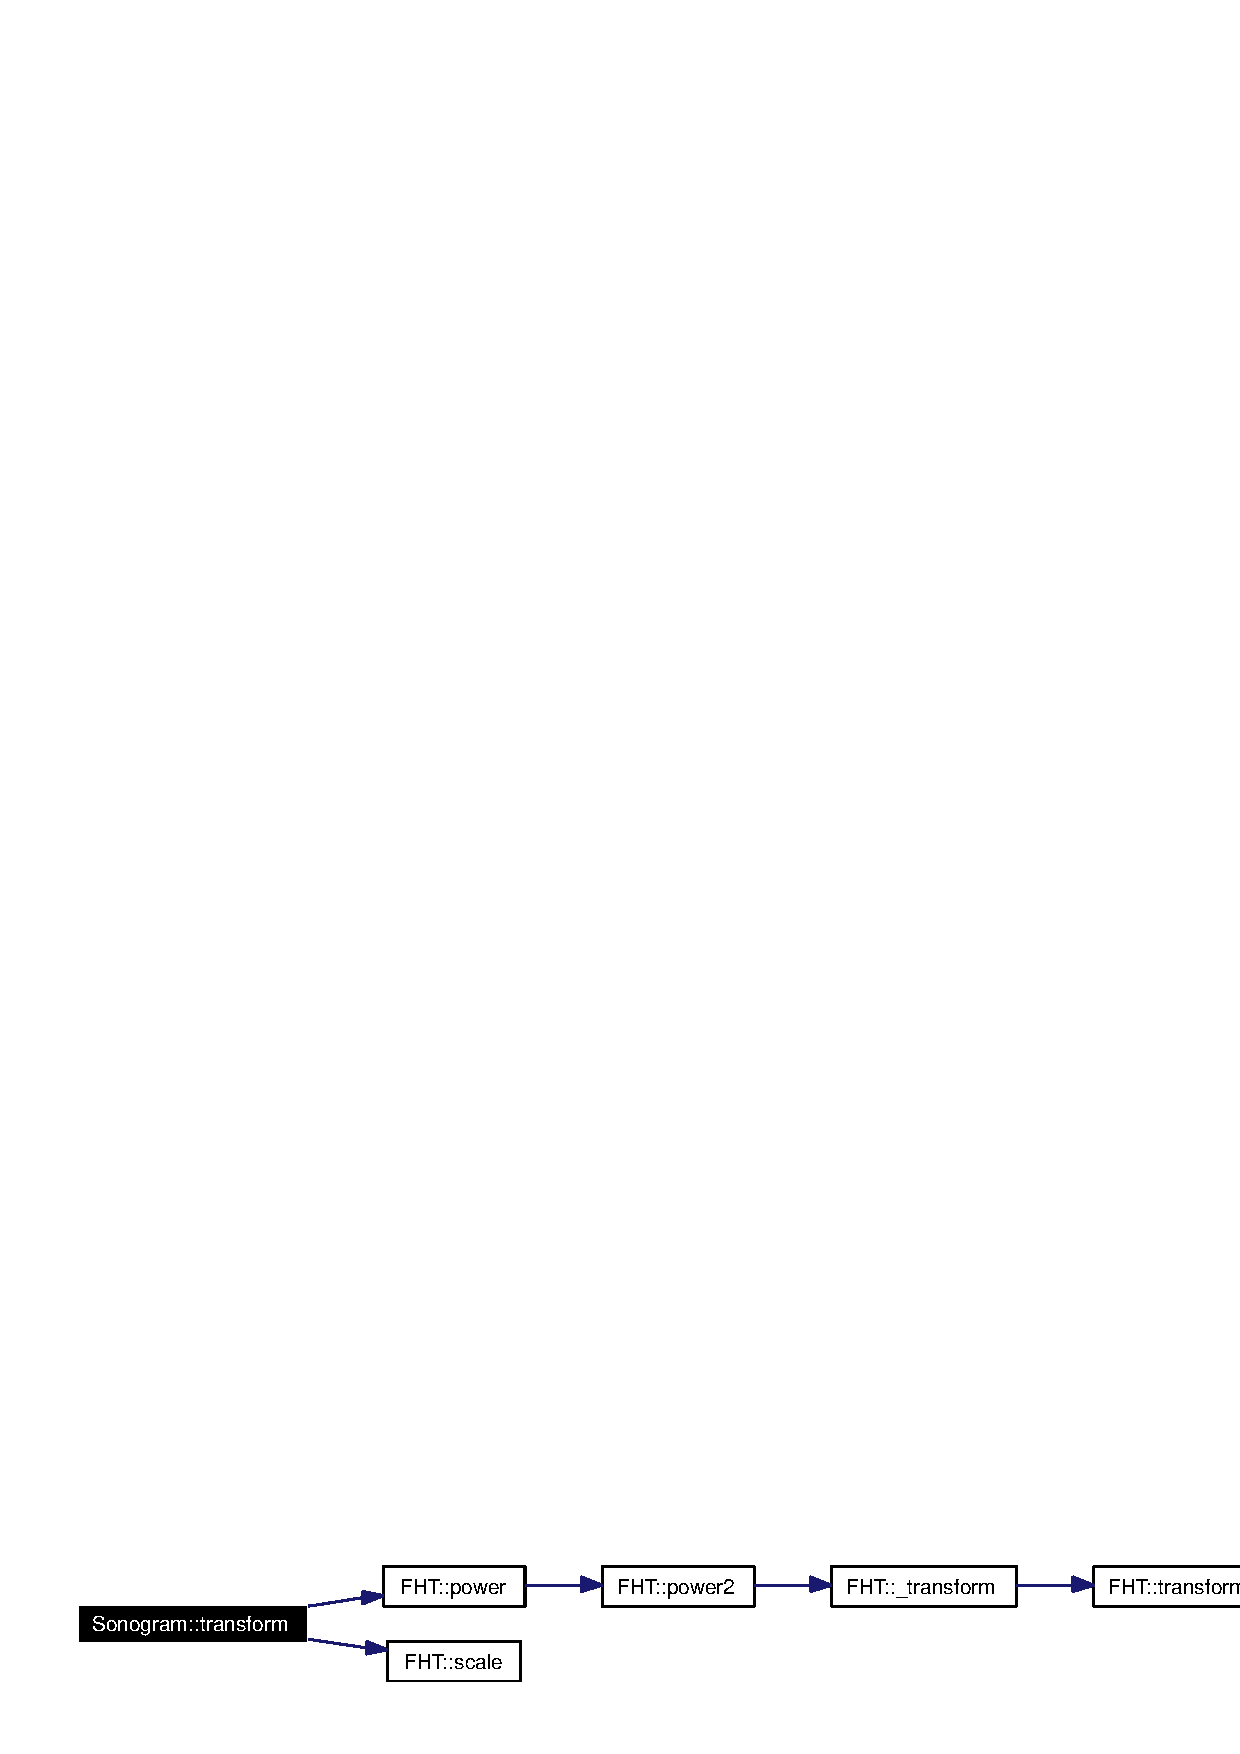
\includegraphics[width=307pt]{classSonogram_Sonograma4_cgraph}
\end{center}
\end{figure}


\subsection{Member Data Documentation}
\index{Sonogram@{Sonogram}!m_fht@{m\_\-fht}}
\index{m_fht@{m\_\-fht}!Sonogram@{Sonogram}}
\subsubsection{\setlength{\rightskip}{0pt plus 5cm}{\bf FHT} {\bf Analyzer::Base}$<$ {\bf QWidget}  $>$::{\bf m\_\-fht}\hspace{0.3cm}{\tt  [protected, inherited]}}\label{classAnalyzer_1_1Base_Analyzer_1_1Basep3}




Definition at line 67 of file analyzerbase.h.\index{Sonogram@{Sonogram}!m_height@{m\_\-height}}
\index{m_height@{m\_\-height}!Sonogram@{Sonogram}}
\subsubsection{\setlength{\rightskip}{0pt plus 5cm}uint {\bf Analyzer::Base}$<$ {\bf QWidget}  $>$::{\bf m\_\-height}\hspace{0.3cm}{\tt  [protected, inherited]}}\label{classAnalyzer_1_1Base_Analyzer_1_1Basep2}




Definition at line 66 of file analyzerbase.h.\index{Sonogram@{Sonogram}!m_timeout@{m\_\-timeout}}
\index{m_timeout@{m\_\-timeout}!Sonogram@{Sonogram}}
\subsubsection{\setlength{\rightskip}{0pt plus 5cm}uint {\bf Analyzer::Base}$<$ {\bf QWidget}  $>$::{\bf m\_\-timeout}\hspace{0.3cm}{\tt  [protected, inherited]}}\label{classAnalyzer_1_1Base_Analyzer_1_1Basep1}




Definition at line 65 of file analyzerbase.h.\index{Sonogram@{Sonogram}!m_timer@{m\_\-timer}}
\index{m_timer@{m\_\-timer}!Sonogram@{Sonogram}}
\subsubsection{\setlength{\rightskip}{0pt plus 5cm}QTimer {\bf Analyzer::Base}$<$ {\bf QWidget}  $>$::{\bf m\_\-timer}\hspace{0.3cm}{\tt  [protected, inherited]}}\label{classAnalyzer_1_1Base_Analyzer_1_1Basep0}




Definition at line 64 of file analyzerbase.h.

The documentation for this class was generated from the following files:\begin{CompactItemize}
\item 
{\bf sonogram.h}\item 
{\bf sonogram.cpp}\end{CompactItemize}
